\chapter{环境配置}
\section{CMake}
	\subsection{简介}
	\par CMake是个开源的跨平台自动化建构系统,它用配置文件控制建构过程(build process)的方式和Unix的Make相似,只是CMake的配置文件取名为CMakeLists.txt。Cmake并不直接建构出最终的软件,而是产生标准的建构档(如Unix的Makefile或Windows Visual C++的projects/workspaces),然后再依一般的建构方式使用。这使得熟悉某个集成开发环境(IDE)的开发者可以用标准的方式建构他的软件,这种可以使用各平台的原生建构系统的能力是CMake和SCons等其他类似系统的区别之处。CMake可以编译源代码、制做程序库、产生适配器(wrapper)、还可以用任意的顺序建构可执行文件。CMake支持in-place建构(二进档和源代码在同一个目录树中)和out-of-place建构(二进档在别的目录里),因此可以很容易从同一个源代码目录树中建构出多个二进档。CMake也支持静态与动态程序库的建构。\cite{ wiki:CMake}
	\subsection{安装}
	\par CMake要求每个目录下均有一个CMakeLists.txt文件,一个通用的目录结构如下:
	\dirtree{%
	.1 ..
	.2 app.
	.3 CMakeLists.txt.
	.3 main.cc.
	.3 main.h.
	.2 include.
	.3 CMakeLists.txt.
	.3 test.h.
	.2 lib.
	.3 test\_impl.cc.
	.3 test\_impl.h.
	.2 CMakeLists.txt.
	.2 README.md.	
	}
	\par\noindent 其中:\\
	\par\noindent \lstinline[language=sh]{app}目录下放置\lstinline[language=sh]{main}函数所在文件,可以同时包含多个将要生成的程序,最终将在\lstinline[language=sh]{./build/app/}目录下生成与该文件同名的可执行文件,在\lstinline[language=sh]{./build/app/}目录下执行\lstinline[language=sh]{./main}即可运行。
	\par\noindent \lstinline[language=sh]{include}目录下放置头文件。
	\par\noindent \lstinline[language=sh]{lib}目录下为需要该项目生成的库文件。
	\par\noindent \lstinline[language=sh]{README.md}为用Markdown书写的说明文档。
\section{Boost C++ Libraries}
	\subsection{简介}
	\par Boost C++ 库(Libraries)是一组扩充C++功能的经过同行评审(Peer-reviewed)且开放源代码程序库。大多数的函数为了能够以开放源代码、封闭项目的方式运作,而授权于Boost软件许可协议(Boost Software License)之下。许多Boost的开发人员是来自C++标准委员会,而部分的Boost库成为C++的TR1标准之一。
	\par 为了要确保库的效率与弹性,Boost广泛的使用模板(template)功能。而它是针对各式领域的C++用户与应用领域(Application Domain)上,包含的库类别从像smart\_ptr 库这种类通用库,到像是文件系统的操作系统抽象层,甚至能够利用Boost来开发额外的库或是给高级的C++用户利用,像是MPL。\cite{ wiki:Boost}
\section{Doxygen}
	\subsection{简介}
	\par Doxygen是一个C++、C、Java、Objective-C、Python、IDL(CORBA和Microsoft flavors)、Fortran、VHDL、PHP、C\#和D语言的文檔生成器。可以在大多数类Unix的系统上运行,以及Mac OS X操作系统和Microsoft Windows。初始版本的Doxygen使用了一些旧版本DOC++的源代码;随后,Doxygen源代码由Dimitri van Heesch重写。
	\par Doxygen是一个编写软件参考文檔的工具。该文檔是直接写在源代码中,因此比较容易保持更新。Doxygen可以交叉引用文檔和源代码,使文件的读者可以很容易地引用实际的源代码。
	\par KDE使用Doxygen作为其部分文档且KDevelop具有内置的支持。 Doxygen的发布遵守GNU通用公共许可证,并且是自由软件。\cite{ wiki:Doxygen}
\section{Python}
	\subsection{简介}
	\par Python,是一种面向对象、解释型的计算机程序语言。它包含了一组功能完备的标准库,能够轻松完成很多常见的任务。它的语法简单,与其它大多数程序设计语言使用大括号不一样,它使用缩进来定义语句块。
	\par 与Scheme、Ruby、Perl、Tcl等动态语言一样,Python具备垃圾回收功能,能够自动管理内存使用。它经常被当作脚本语言用于处理系统管理任务和网络程序编写,然而它也非常适合完成各种高级任务。Python虚拟机本身几乎可以在所有的作业系统中运行。使用一些诸如py2exe、PyPy、PyInstaller之类的工具可以将Python源代码转换成可以脱离Python解释器运行的程序。
	\par Python的官方解释器是CPython,该解释器用C语言编写,是一个由社区驱动的自由软件,目前由Python软件基金会管理。
	\par Python支持命令式程序设计、面向对象程序设计、函数式编程、面向侧面的程序设计、泛型编程多种编程范式。\cite{ wiki:Python}
\section{SWIG}
	\subsection{简介}
	\par SWIG是个帮助使用C或者C++编写的软件能与其它各种高级编程语言进行嵌入联接的开发工具。SWIG能应用于各种不同类型的语言包括常用脚本编译语言例如Perl, PHP, Python, Tcl, Ruby and PHP。支持语言列表中也包括非脚本编译语言,例如C\#, Common Lisp (CLISP, Allegro CL, CFFI, UFFI), Java, Modula-3, OCAML以及R,甚至是编译器或者汇编的计划应用(Guile, MzScheme, Chicken)。SWIG普遍应用于创建高级语言解析或汇编程序环境,用户接口,作为一种用来测试C/C++或进行原型设计的工具。SWIG还能够导出XML或Lisp s-expressions格式的解析树。SWIG可以被自由使用,发布,修改用于商业或非商业中。\cite{ wiki:SWIG}
\section{USRP}
	\subsection{简介}
	\par Universal Software Radio Peripheral (USRP) is a range of software-defined radios designed and sold by Ettus Research and its parent company, National Instruments. Developed by a team led by Matt Ettus, the USRP product family is intended to be a comparatively inexpensive hardware platform for software radio, and is commonly used by research labs, universities, and hobbyists.
	\par Most USRPs connect to a host computer through a high-speed link, which the host-based software uses to control the USRP hardware and transmit/receive data. Some USRP models also integrate the general functionality of a host computer with an embedded processor that allows the USRP device to operate in a stand-alone fashion.
	\par The USRP family was designed for accessibility, and many of the products are open source hardware. The board schematics for select USRP models are freely available for download; all USRP products are controlled with the open source UHD driver, which is free and open source software. USRPs are commonly used with the GNU Radio software suite to create complex software-defined radio systems. \cite{ wiki:USRP}
	% TODO:translate
\section{HackRF}
	\subsection{简介}
	\par HackRF是一款由Michael Ossmann发起的开源软件无线电外设,旨在从30MHz到6GHz,于2012年从DARPA处拿了一笔经费,制作了500块测试版本Jawbreaker,并向社会分发测试。在经过用户对Jawbreaker的反馈后,作者对硬件板卡做了重新布线,改善了射频性能,这一点我们将会在后文详细讨论。 随后于2013年7月31日至9月4日共计35天的时间,在著名的社会化融资平台Kickstarter上,迅速地获得多达1991人的预订,共预订出价值为\$602,960的HackRF One。
	\begin{figure}[htb]
	\centering
	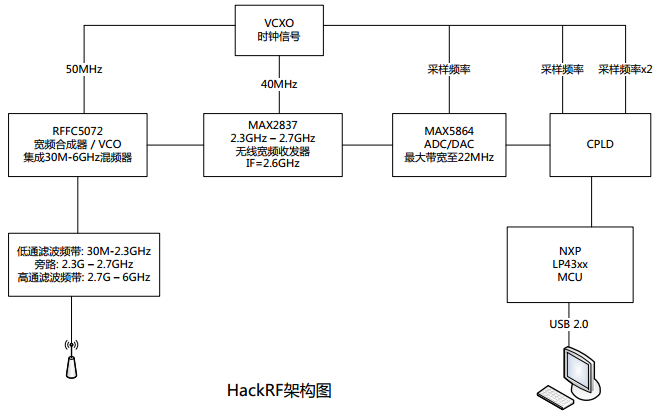
\includegraphics{figures/HackRF_架构.png}
	\caption{
		HackRF\_架构图
	}
	\label{fig:HackRF_架构}
	\end{figure}
	\subsection{osmosdr}
\section{gqrx}
	\subsection{简介}
\section{git}
	\subsection{简介}
	\par git是用于Linux内核开发的版本控制工具。与CVS、Subversion一类的集中式版本控制工具不同,它采用了分布式版本库的作法,不需要服务器端软件,就可以运作版本控制,使得源代码的发布和交流极其方便。git的速度很快,这对于诸如Linux内核这样的大项目来说自然很重要。git最为出色的是它的合并追踪(merge tracing)能力。  
	\par 实际上内核开发团队决定开始开发和使用git来作为内核开发的版本控制系统的时候,世界上开源社区的反对声音不少,最大的理由是git太艰涩难懂,从git的内部工作机制来说,的确是这样。但是随着开发的深入,git的正常使用都由一些友善的命令稿来执行,使git变得非常好用。现在,越来越多的著名项目采用git来管理项目开发,例如:wine、U-boot等。  
	\par 作为开源自由原教旨主义项目,git没有对版本库的浏览和修改做任何的权限限制,通过其他工具也可以达到有限的权限控制,比如:gitosis、CodeBeamer MR。原本git的使用范围只适用于Linux/Unix平台,但在Windows平台下的使用也日渐成熟,这主要归功于Cygwin、msysgit环境,以及TortoiseGit这样易用的GUI工具。git的源代码中也已经加入了对Cygwin与MinGW编译环境的支持且逐渐完善,为Windows用户带来福音。
	\subsection{常用命令}
	\par 在众多教程中,廖雪峰的官方网站(\href{http://www.liaoxuefeng.com/}{http://www.liaoxuefeng.com/})很适合初学者,深入浅出的讲解了使用git过程中常用的许多命令。
	\subsection{版本控制}
	\subsection{github}
	\par GitHub是一个通过Git进行版本控制的软件源代码托管服务,由GitHub公司(曾称Logical Awesome)的开发者Chris Wanstrath、PJ Hyett和Tom Preston-Werner使用Ruby on Rails编写而成。
	\par GitHub同时提供付费账户和免费账户。这两种账户都可以创建公开的代码仓库,但是付费账户还可以创建私有的代码仓库。根据在2009年的Git用户调查,GitHub是最流行的Git访问站点。除了允许个人和组织创建和访问保管中的代码以外,它也提供了一些方便社会化共同软件开发的功能,即一般人口中的社区功能,包括允许用户追踪其他用户、组织、软件库的动态,对软件代码的改动和bug提出评论等。GitHub也提供了图表功能,用于概观显示开发者们怎样在代码库上工作以及软件的开发活跃程度。
	\par 截止到2015年,GitHub已经有超过九百万注册用户和2110万代码库。事实上已经成为了世界上最大的代码存放网站和开源社区。\cite{ wiki:GitHub}
	\par 本设计使用的众多开源库、软件均已托管于GitHub,网址如下:
	\begin{itemize}
		\item gnuradio/gnuradio\\\href{https://github.com/gnuradio/gnuradio}{https://github.com/gnuradio/gnuradio}
		\item gnuradio/pybombs\\\href{https://github.com/gnuradio/pybombs}{https://github.com/gnuradio/pybombs}
		\item EttusResearch/uhd\\\href{https://github.com/EttusResearch/uhd}{https://github.com/EttusResearch/uhd}
		% TODO:add all github
	\end{itemize}
\section{Docker}
	\subsection{简介}
	\par Docker是一个开放源代码软件项目,让应用程序布署在软件容器下的工作可以自动化进行,借此在Linux操作系统上,提供一个额外的软件抽象层,以及操作系统层虚拟化的自动管理机制。Docker利用Linux核心中的资源分脱机制,例如cgroups,以及Linux核心名字空间(name space),来创建独立的软件容器(containers)。这可以在单一Linux实体下运作,避免引导一个虚拟机造成的额外负担。Linux核心对名字空间的支持完全隔离了工作环境中应用程序的视野,包括进程树、网络、用户ID与挂载文件系统,而核心的cgroup提供资源隔离,包括CPU、存储器、block I/O与网络。从0.9版本起,Dockers在使用抽象虚拟是经由libvirt的 LXC与systemd - nspawn提供界面的基础上,开始包括libcontainer库做为以自己的方式开始直接使用由Linux核心提供的虚拟化的设施,
	\par 依据行业分析公司“451研究”:“Dockers是有能力打包应用程序及其虚拟容器,可以在任何Linux服务器上运行的依赖性工具,这有助于实现灵活性和便携性,应用程序在任何地方都可以运行,无论是公有云、私有云、单机等。”\cite{ wiki:Docker} 
	\par 在构建应用时,如果在实机上进行运行测试,很容易因为依赖的问题导致应用无法正常运行,严重时会造成系统的崩溃。Docker提供了一个虚拟的环境来构建自己的应用,同时也能够与git进行版本控制,与回滚,在Docker中构建应用也能更快的部署应用。需要大规模部署应用时只需要从仓库中拉取自己需要的环境以及版本即可,进行少量的配置即可运行。
	\subsection{构建容器}
\section{GNU Radio}
	\subsection{简介}
	\begin{itemize}
		\item 源码编译
		\item apt-get
			\begin{itemize}
				\item 树莓派
				\par jessie源中提供的GNU Radio版本为3.7.5。
				\par 使用jessie源时需要手动编译gr-dvbt并链接动态库。
				\par stretch源中提供的GNU Radio版本为3.7.10。
				\par 如果需要使用stretch源则需要修改source.list文件。
				\item Ubuntu
			\end{itemize}
		\item pybombs安装
	\end{itemize}
	\subsection{版本选择}
		\begin{itemize}
			\item GNU Radio 3.7.9及以下版本gr-dvbt编译
				\begin{itemize}
					\item x86平台编译
					\item arm平台编译
					\par 由于gr-dvbt中viterbi解码模块使用了汇编,调用了x86平台上的汇编库来加速运算,所以在arm平台无法编译viterbi模块,也就导致了仅能在arm平台上编译发射端的部分。
					\par 需要注释以下文件中的以下语句:
					% TODO:汇编注释
				\end{itemize}
			\item GNU Radio 3.7.10
				\par 安装完成之后使用python测试,gnuradio需要Python 2,在Python3环境下无法运行。
\begin{lstlisting}[ language= sh ]
Python 2.7.13 (default, Jan 19 2017, 14:48:08) 
[GCC 6.3.0 20170118] on linux2
Type "help", "copyright", "credits" or "license" for more information.
>>> import gnuradio
>>> 
\end{lstlisting}
				\par 如果没有出现\lstinline[language=sh]{no module named gnuradio}则表示安装成功。
		\end{itemize}
\endinput